\subsection{Differential branching fraction}
\label{sec:kpimm:bf}
 
The differential branching fraction $\deriv\BF/\deriv\qsq$ of the decay \BdToKpimm in an interval ($q^{2}_{\text{min}}$, $q^{2}_{\text{max}}$) is given by

\begin{equation}
\begin{split}
\frac{\deriv\BF}{\deriv\qsq} = \frac{1}{(q^{2}_{\text{max}} - q^{2}_{\text{min}}) }&f_{\KstP}\BF(\BdToJPsiKstP)\BF(\decay{\jpsi}{\mumu}) \\
\times&\BF(\decay{\KstP}{\Kp\pim})\frac{N'_{\kpimm}}{(1-F_{\rm S}^{\jpsi\Kstarz})N'_{\jpsi\Kstarz}},
\end{split}
\label{eqn:dbfdq2}
\end{equation}

\noindent where $N'_{\kpimm}$ and $N'_{\jpsi\Kstarz}$ are the acceptance-corrected yields of the \BdToKpimm and \BdToJPsiKst decays, respectively. The \BdToJPsiKst yield has to be corrected for the S-wave fraction within the narrow $\mkpi$ window of \BdToJPsiKst decays, $F_{\rm S}^{\jpsi\Kstarz}$. The value of $F_{\rm S}^{\jpsi\Kstarz}$ is obtained from Ref.~\cite{LHCb-PAPER-2013-023} and is recalculated for the $\mkpi$ range $796<\mkpi<996~\mevcc$. The branching fractions $\BF(\BdToJPsiKstP)$, $\BF(\decay{\jpsi}{\mumu})$ and $\BF(\decay{\KstP}{\Kp\pim})$ are $(1.19\pm0.01\pm0.08)\times10^{-3}$~\cite{belle-z-paper}, $(5.961 \pm 0.033) \times 10^{-2}$~\cite{pdg} and 2/3, respectively. The fraction $f_{\KstP}$ is used to scale the value of $\BF(\BdToJPsiKstP)$ to the appropriate \mkpi range and is calculated by integrating the $\KstP$ line shape given in Ref.~\cite{belle-z-paper} over the range $796<\mkpi<996~\mevcc$.
 
\subsubsection{Acceptance corrected yields}
 
To avoid making any assumptions about the unknown distributions of the \BdToKpimm candidates, the event-by-event efficiencies described in Sec.~\ref{sec:kpimm:acceptance} are used to correct the measured yields by calculating the average acceptance weight, where each weight is the reciprocal of the event-by-event efficiency.
 
For the case where there are only signal candidates present, the average weight would simply be calculated as,
 
\begin{equation}
\overline{w} = \frac{1}{N}\sum\limits_{i}^{N}w_{i},
\label{eqn:average_eff}
\end{equation}
 
\noindent where $w_{i}$ is the event-by-event acceptance and $N$ is the number of candidates.  An estimate for the error on the average weight is given by,
 
\begin{equation}
\delta_{\overline{w}} = \sqrt{\frac{1}{N(N-1)}\sum\limits_{i}^{N}(w_{i}-\overline{w})^{2}}.
\end{equation}
 
Due to the presence of background, the average weight calculated in the signal mass window will be an admixture of the average weight for both signal candidates ($\overline{w}_{sig}$) and background candidates ($\overline{w}_{bkg}$),
 
\begin{equation}
\overline{w}_{mix} = \frac{N_{sig}\overline{w}_{sig} + N_{bkg}\overline{w}_{bkg}}{N_{sig}+N_{bkg}},
\end{equation}
 
\noindent where $N_{sig}$ and $N_{bkg}$ are the number of signal and background events in the signal mass window, respectively. This can be rearranged to give the average weight for the signal candidates,
 
\begin{equation}
\overline{w}_{sig} = \frac{(N_{sig}+N_{bkg})\overline{w}_{mix} -  N_{bkg}\overline{w}_{bkg}}{N_{sig}}.
\end{equation}
 
However, what is needed for both \BdToKpimm and \BdToJPsiKst is the acceptance corrected yield $\overline{w}_{sig}N_{sig}$.  This is given by,
 
\begin{equation}
\overline{w}_{sig}N_{sig} = (N_{sig}+N_{bkg})\overline{w}_{mix} -  N_{bkg}\overline{w}_{bkg}
\end{equation}
 
\noindent where the errors are propagated as,
 
\begin{equation}
\begin{split}
\sigma_{\overline{w}_{sig}N_{sig}}^{2} =~ &(N_{sig}+N_{bkg})^{2}\sigma_{\overline{w}_{mix}}^{2} + (-N_{bkg})^{2}\sigma_{\overline{w}_{bkg}}^{2}\\
&+(\overline{w}_{mix})^{2}\sigma_{N_{sig}}^{2} + (\overline{w}_{mix}-\overline{w}_{bkg})^{2}\sigma_{N_{bkg}}^{2}.
\end{split}
\end{equation}
 
The signal region is defined as $5230<\mkpimm<5330$~\mevcc and the background region as $5350<\mkpimm<5700$~\mevcc. For the resonant mode, the background region is altered to $5450<\mkpimm<5700$~\mevcc in order to prevent any potential pollution from \BdToJPsiKst or \BsToJPsiKst candidates.

\subsubsection{Toy studies}

Toy studies are performed for the extraction of $\overline{w}_{sig}N_{sig}$ with different numbers of signal and background candidates.  In each toy $N_{sig}$, $N_{bkg}$ are Poisson fluctuated.  The nominal mass models, described in Sec.~\ref{sec:kpimm:massfit}, are used to generate signal and background candidates. The weights for both signal and background are sampled from two gaussian functions with different means. 

Pull studies are performed to check that the method is unbiased and correctly estimates the uncertainty. The pull of the observable $a$ is defined as $(a_{\rm meas}-a_{\rm gen})/\sigma(a)_{\rm meas}$~\cite{lyons-pulls}. If the method is unbiased and the coverage is correct, the pull distribution should be a Gaussian centred at zero with unit width. The pulls for the extraction of $\overline{w}_{sig}N_{sig}$ are shown in Fig.~\ref{fig:bf:pulls}. No bias is observed and the statistical error is correctly evaluated.
 
\begin{figure}[!tb]
 \centering
 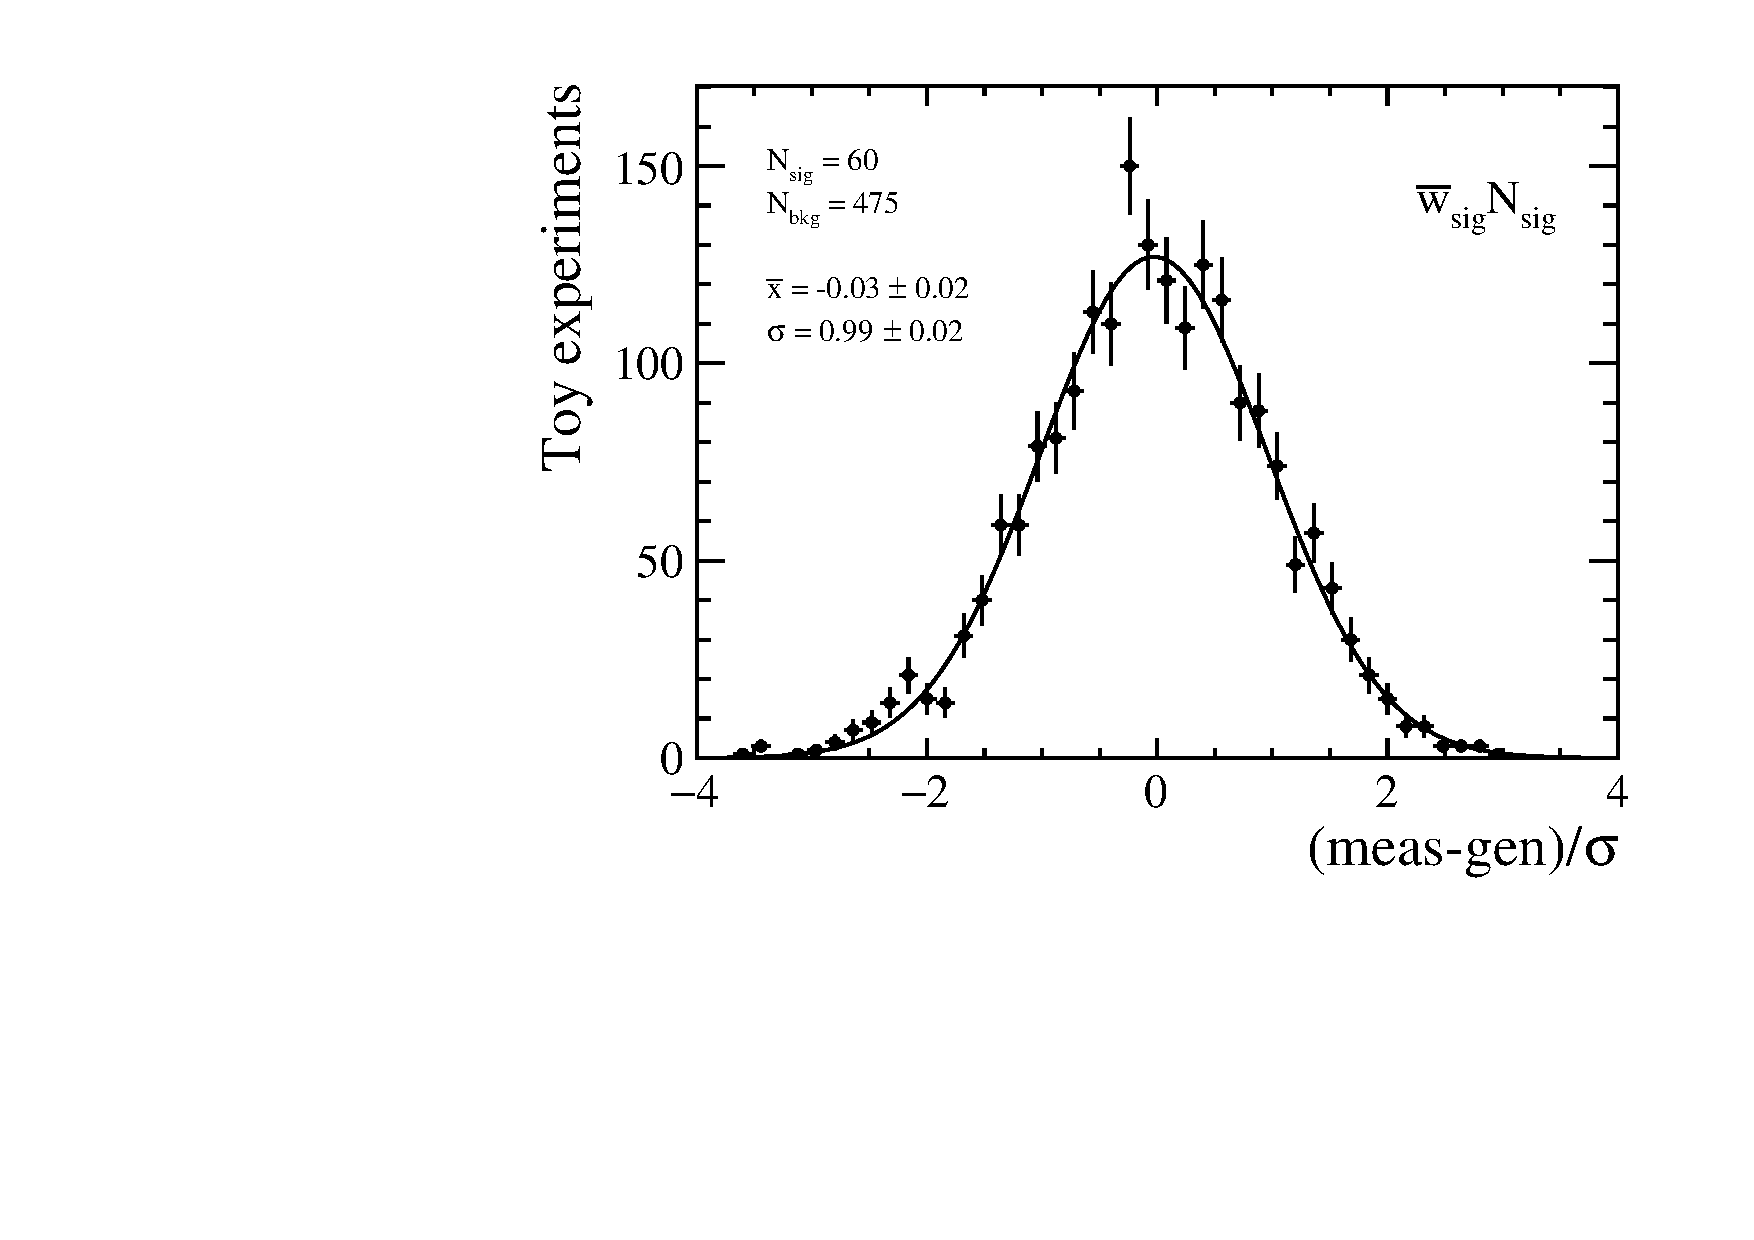
\includegraphics[width=0.45\textwidth]{figs/kpimm/bf/n_prime_low_yield.pdf}
 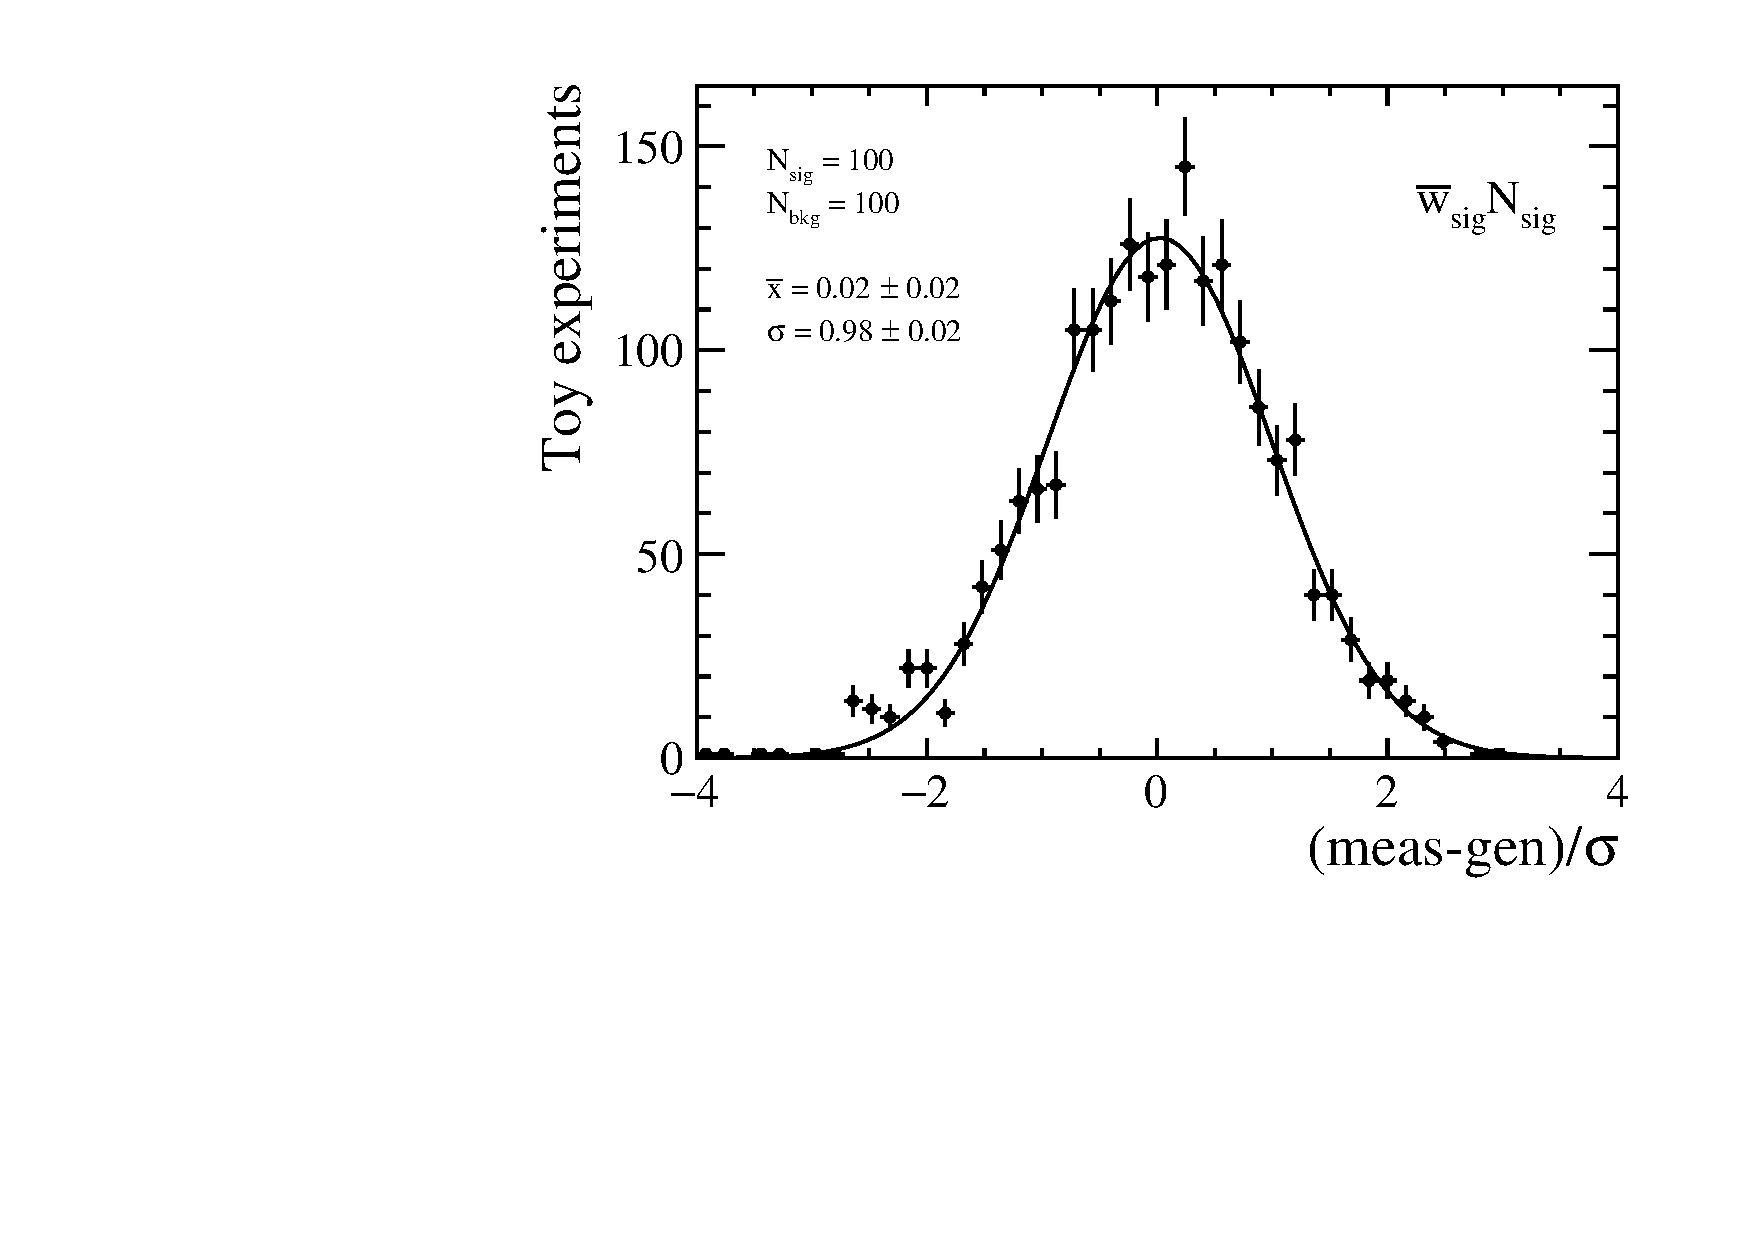
\includegraphics[width=0.45\textwidth]{figs/kpimm/bf/n_prime_med_yield.pdf}
 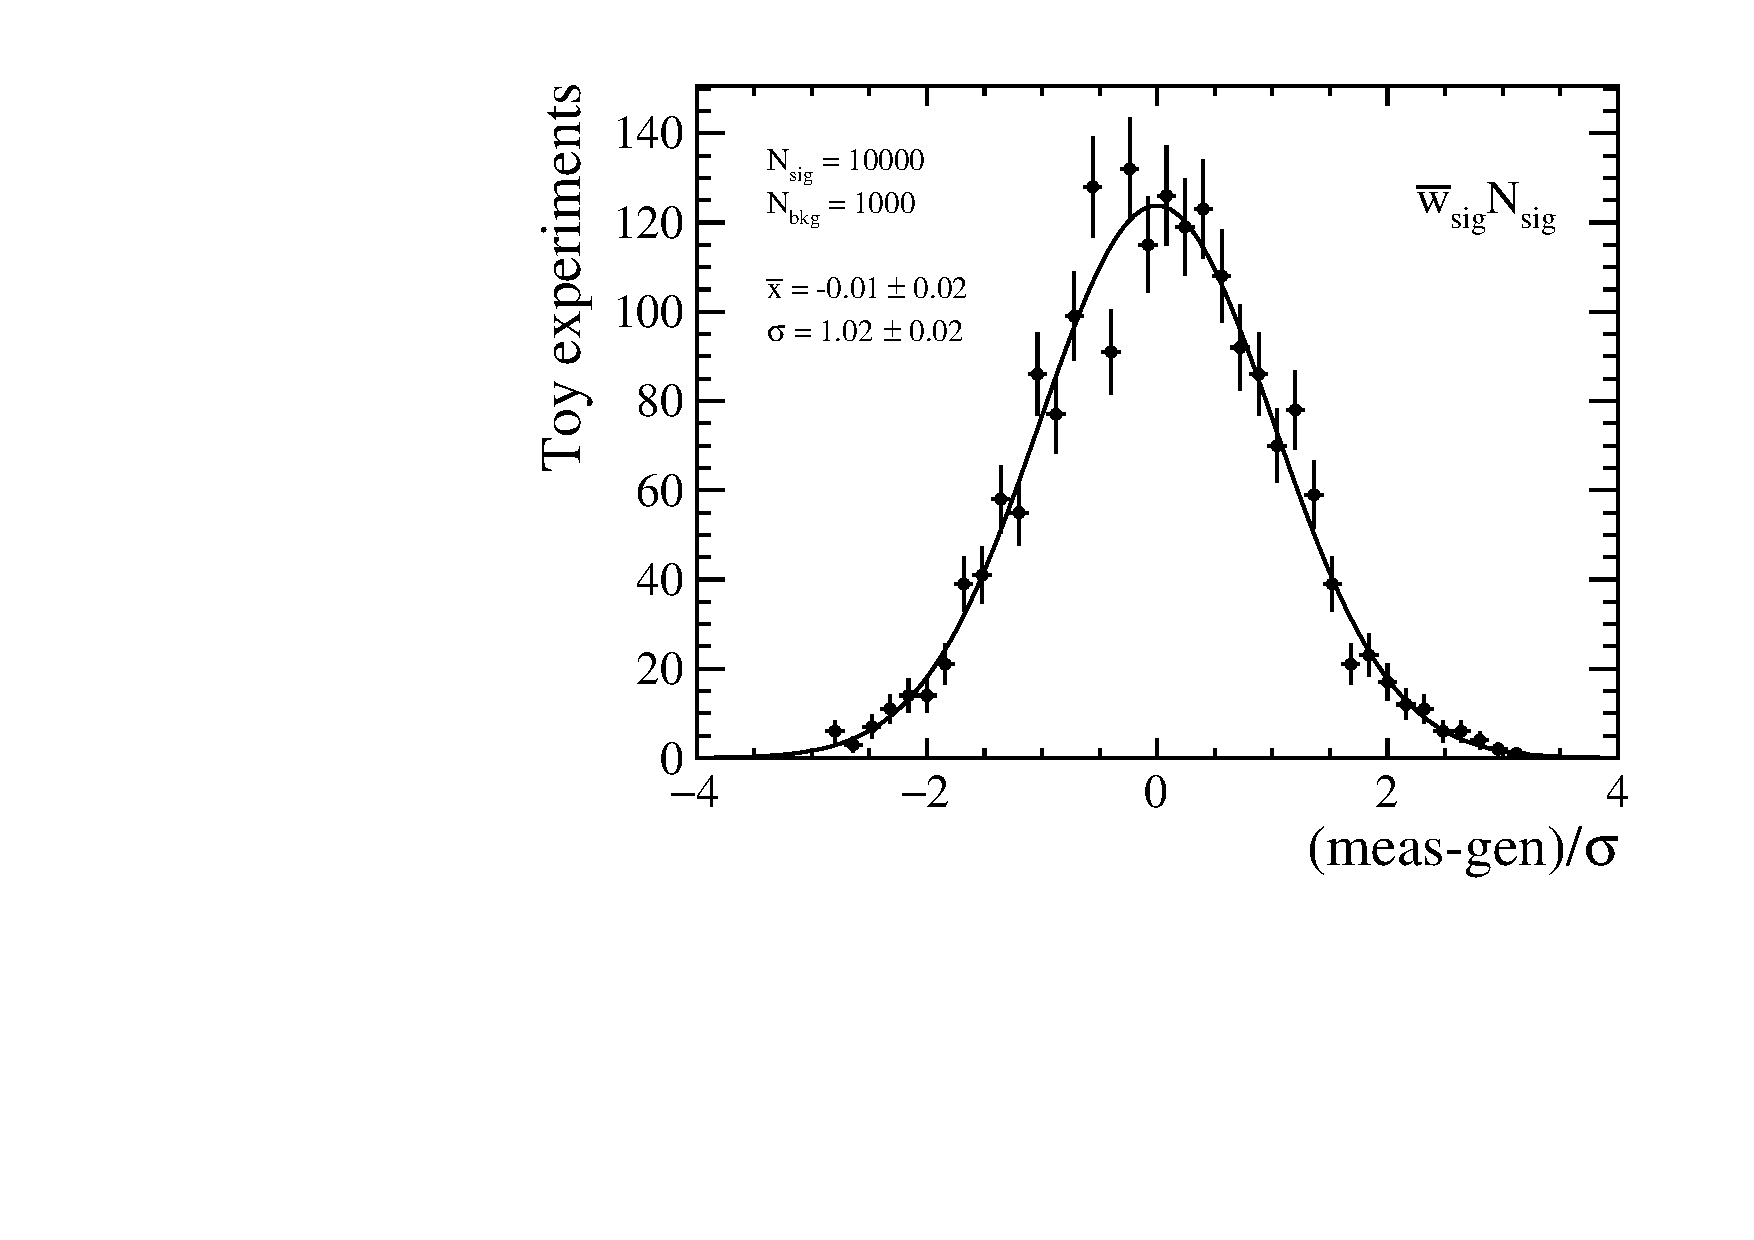
\includegraphics[width=0.45\textwidth]{figs/kpimm/bf/n_prime_high_yield.pdf}
 \caption{Pull plots for the extraction of $\overline{w}_{sig}N_{sig}$ with different numbers of signal and background candidates.}
 \label{fig:bf:pulls}
\end{figure}

\subsubsection{Results}

The results for the differential branching fraction are given in Fig.~\ref{fig:bf}.  The uncertainties shown are the quadratic sum of the statistical and systematic uncertainties.  The results are also presented in Table~\ref{tab:bf}.  The various sources of the systematic uncertainties are described in Sec.~\ref{sec:kpimm:systematics}.
 
\begin{figure}[!tb]
\centering
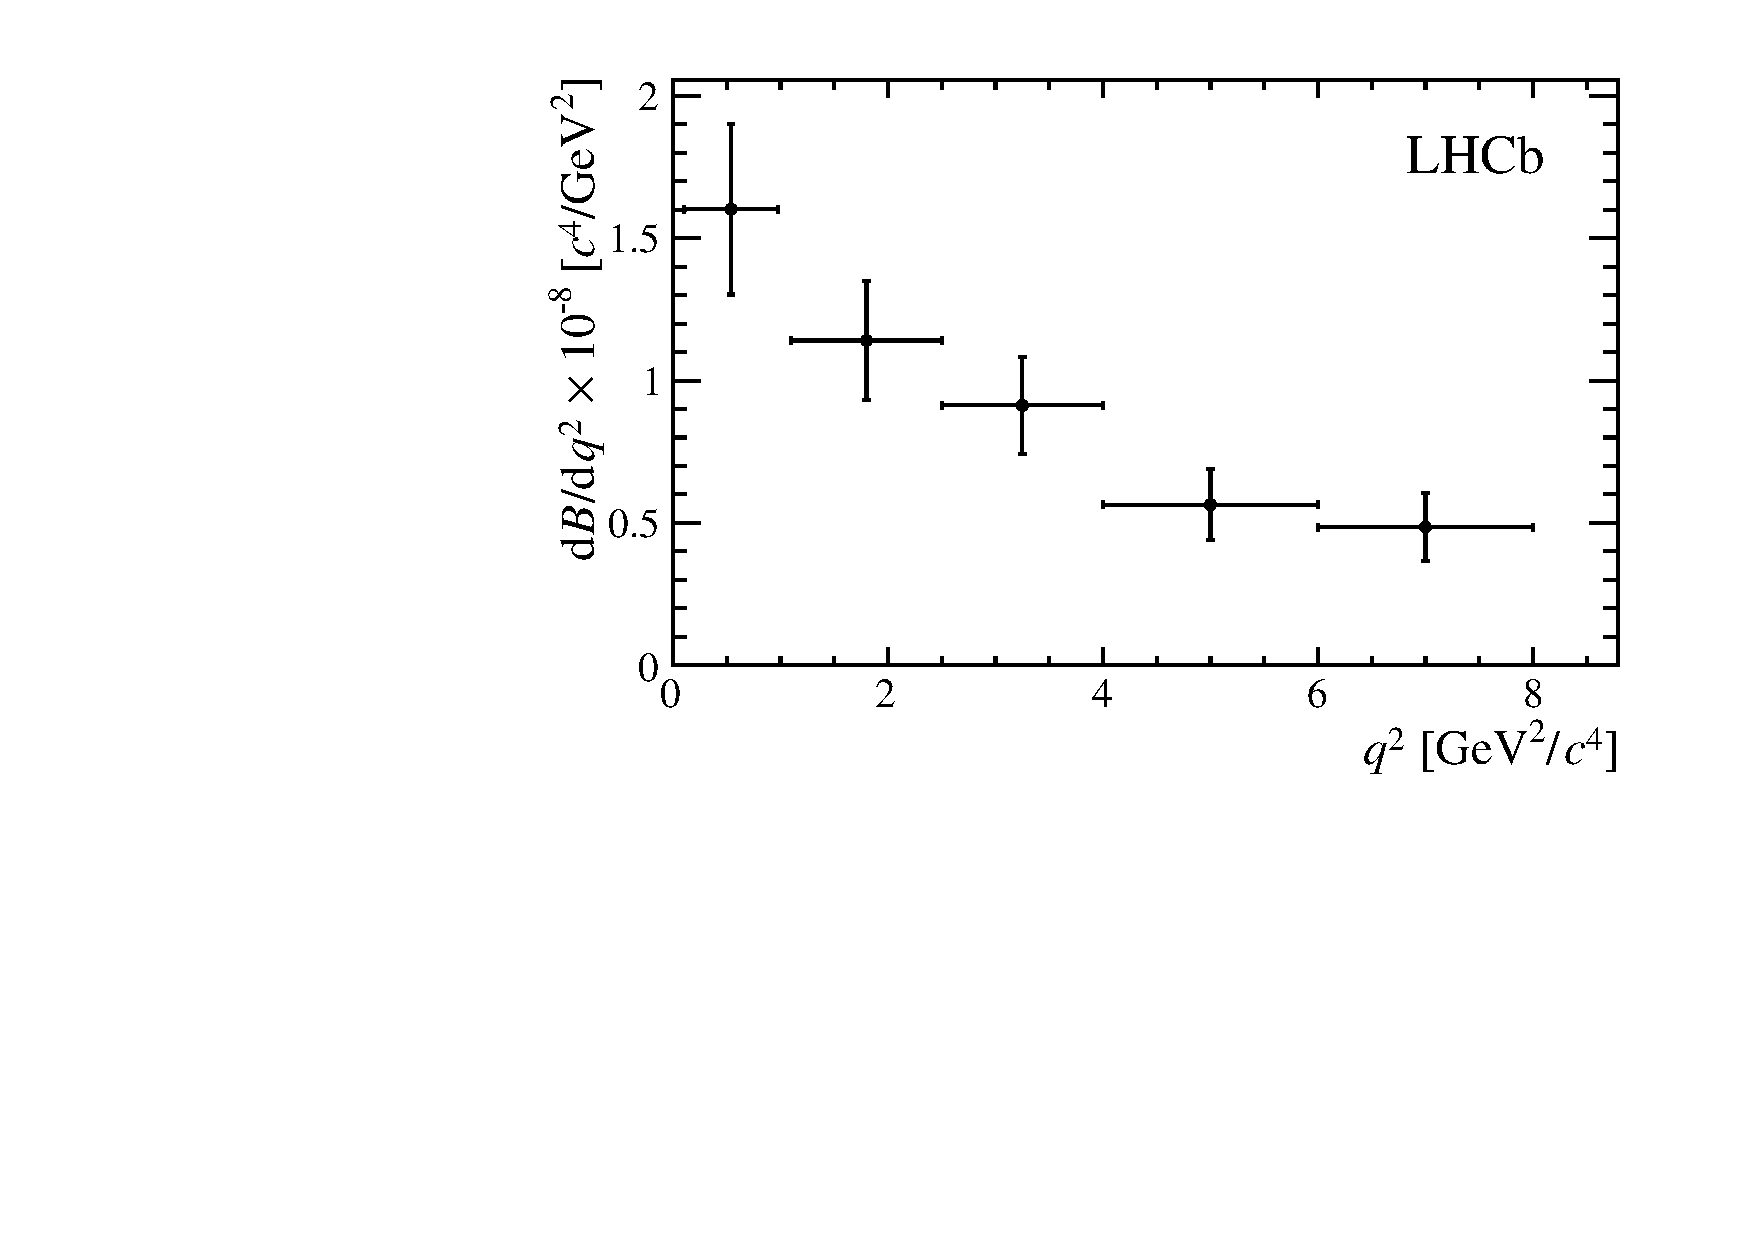
\includegraphics[width=0.7\textwidth]{figs/kpimm/bf/dbfdq2.pdf}
\caption{Differential branching fraction of \BdToKpimm in bins of \qsq. The uncertainties shown are the quadratic sum of the statistical and systematic uncertainties.}
\label{fig:bf}
\end{figure}
 
\begin{table}[!tb]
\caption{Differential branching fraction of \BdToKpimm in bins of \qsq. The first uncertainty is statistical, the second systematic and the third due to the uncertainty on the \BdToJPsiKstP and $\decay{\jpsi}{\mumu}$ branching fractions.}
\label{tab:bf}
\begin{center}
\begin{tabular}{lc}
\qsq [$\gevgevcccc$] & $\deriv\BF/\deriv\qsq \times 10^{-8}~[c^{4}/\gev^{2}]$ \\
\hline
$[0.10,0.98]$ & 1.60 $\pm$ 0.28 $\pm$ 0.04 $\pm$ 0.11 \\
$[1.10,2.50]$ & 1.14 $\pm$ 0.19 $\pm$ 0.03 $\pm$ 0.08 \\
$[2.50,4.00]$ & 0.91 $\pm$ 0.16 $\pm$ 0.03 $\pm$ 0.06 \\
$[4.00,6.00]$ & 0.56 $\pm$ 0.12 $\pm$ 0.02 $\pm$ 0.04 \\
$[6.00,8.00]$ & 0.49 $\pm$ 0.11 $\pm$ 0.01 $\pm$ 0.03 \\
\hline
$[1.10,6.00]$ & 0.82 $\pm$ 0.09 $\pm$ 0.02 $\pm$ 0.06 \\
\end{tabular}
\end{center}
\end{table}